\documentclass[12pt]{article}
\usepackage[utf8]{inputenc}
\usepackage{graphicx}
\graphicspath{ {images/} }
\title{
    {\Huge LANBAC}\\
    {\Large User Documentation}\\
    \vspace{+35pt}
    {
\includegraphics[width=50mm,scale=0.5]{iitb.png}}
}
\author{
    \large Abhishek Sharma 193050054\\
    \large Parmar Raja Vijay 193050090
}
\date{November 27,2019}

\begin{document}
\maketitle
\clearpage
\section*{Instructions}

\begin{enumerate}
    \item Double click on the executable named run.sh.A window should pop up which signifies that the application has started.
    
    \item Select one of the entries depending upon the interface.Entry index starts with 0.Below example shows entry 1 is selected i.e. eno1 interface is selected.
    
    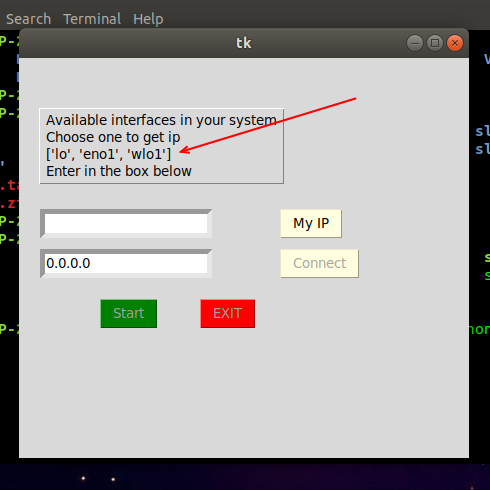
\includegraphics[width=120mm,scale=0.8]{1.png}
    
    \bigbreak
     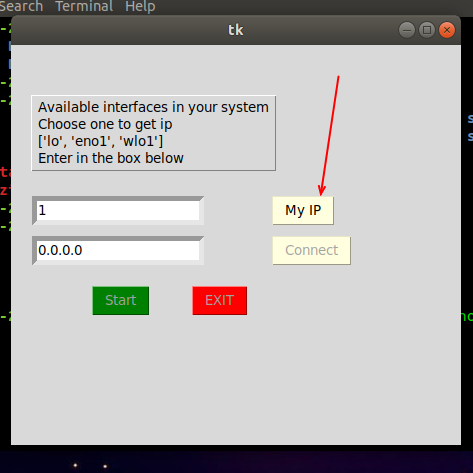
\includegraphics[width=120mm,scale=0.8]{2.png}
     \clearpage
    \item A Diolog box will appear.This shows your IP address.You need to save this IP address and send this to the one who you want to communicate to.After noting the IP address,click OK.
    \bigbreak
     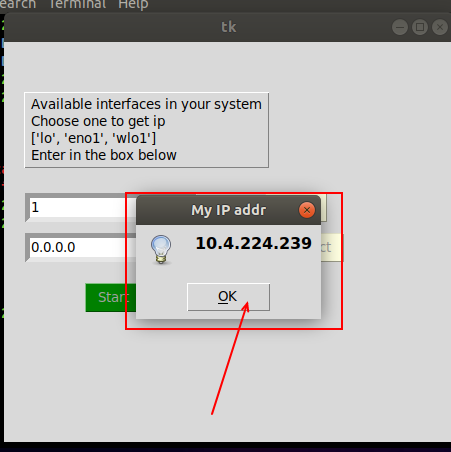
\includegraphics[width=120mm,scale=0.8]{3.png}
     
    \item When you get the IP address from the one who you want to communicate to,enter it in the input box highlighted below and press connect.
    
    \bigbreak
     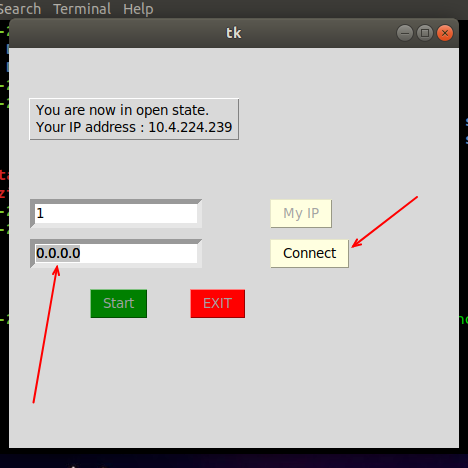
\includegraphics[width=120mm,scale=0.8]{4.png}
     \bigbreak
     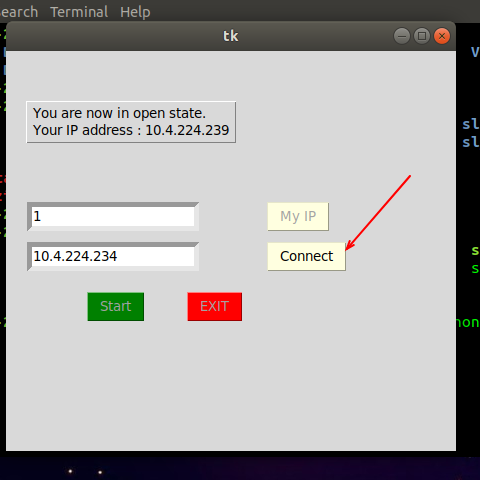
\includegraphics[width=120mm,scale=0.8]{5.png}
     
    \item After pressing Connect,there should be another dialog box which says connected.Press OK.
    
    \bigbreak
     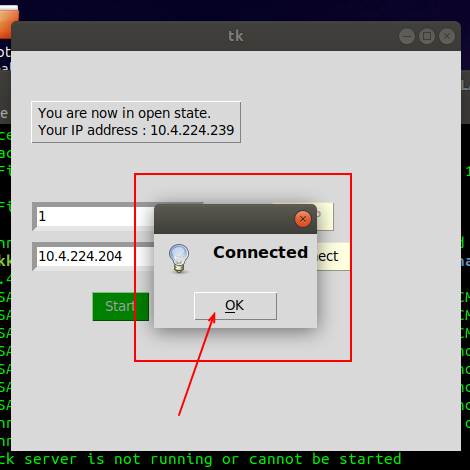
\includegraphics[width=120mm,scale=0.8]{6.png}
     
    \item To start the conversation,press Start button which is highlighted below.A dialog box will appear which says started.It means the conversation and recording of audio has started.You are allowed to speak!
    \bigbreak
     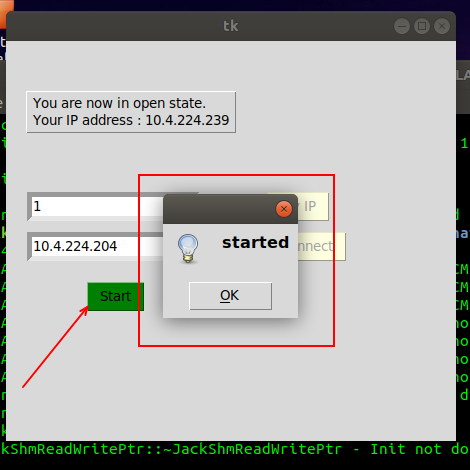
\includegraphics[width=120mm,scale=0.8]{7.png}
     
    \item At any time you are free to exit the conversation.Press Exit to do So as highlighted below.
    
    \bigbreak
     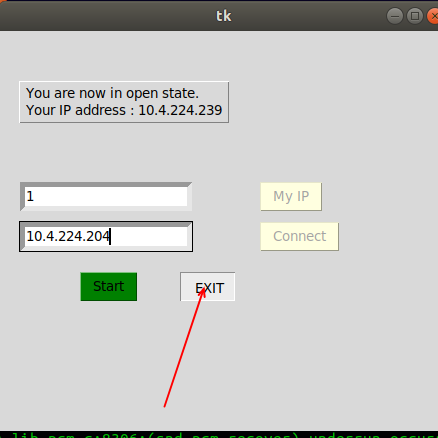
\includegraphics[width=120mm,scale=0.8]{8.png}
\end{enumerate}
\end{document}